\subsection{Ghia's exact solution}
\label{subsec:ghia_exact_solution}

The exact solution for the lid-driven cavity flow at $Re = 1000$ is reported in Ghia et al. \cite{Ghia1982HighReSF}, and it is used as a benchmark to validate the results obtained using our code.

In Ghia's solution, a uniform grid of $129 \times 129$ points is used, and the Reynolds number is imposed as follows:

\begin{equation}
    Re = \begin{cases}
        100 \\
        400 \\
        1000
    \end{cases}
    \rightarrow
    \nu = \frac{U_{lid} L_{domain}}{Re} = \begin{cases}
        0.0100 \\
        0.0025 \\
        0.0010
    \end{cases}
\end{equation}

Where $U_{lid}$ is the velocity of the lid and $L_{domain}$ is the characteristic dimension of the domain.

For reference, in Figure \ref{fig:ghia_solutions} and Figure \ref{fig:ghia_solution_Re1000} we report the solution from Ghia et al. \cite{Ghia1982HighReSF} for the lid-driven cavity flow varying the Reynolds number.

\begin{figure}[H]
    \centering
    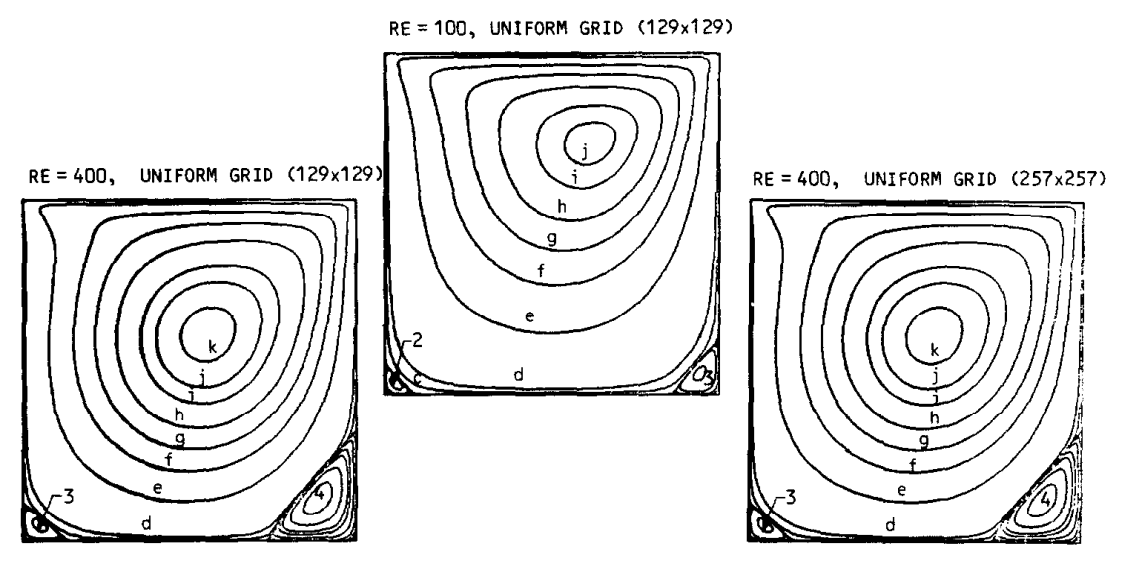
\includegraphics[width=.9\textwidth]{./img/ghia_solutions}
    \caption{Ghia's solutions for the lid-driven cavity flow at different Reynolds numbers.}
    \label{fig:ghia_solutions}
\end{figure}

\begin{figure}[H]
    \centering
    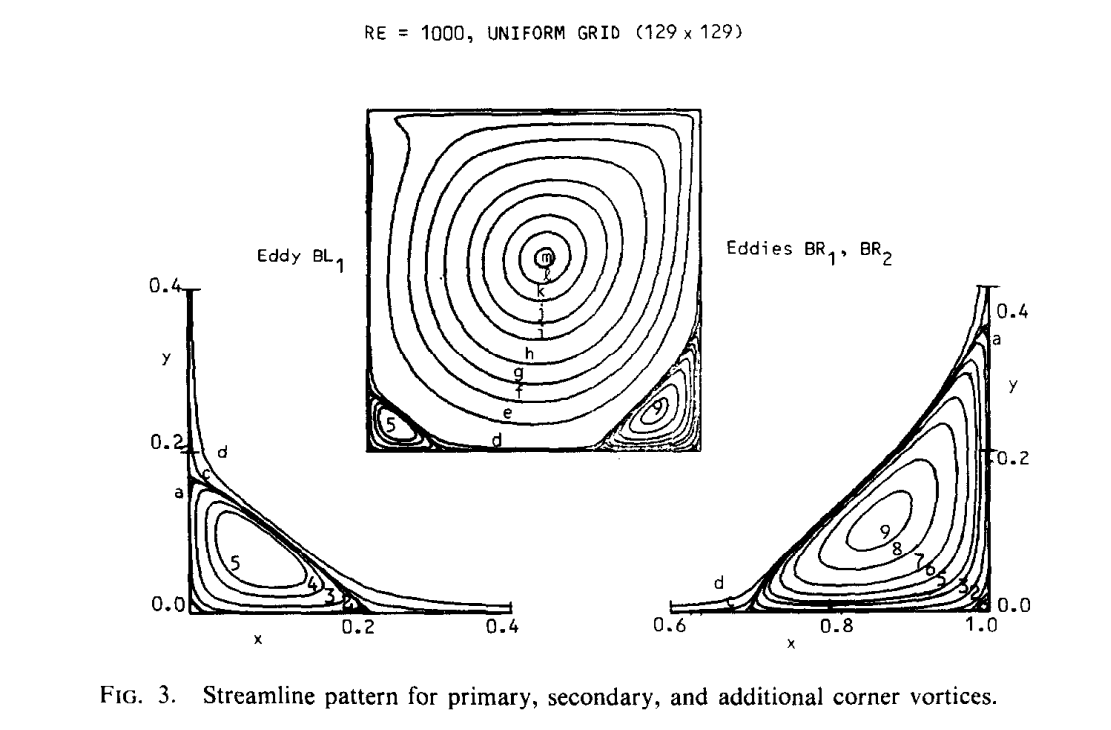
\includegraphics[width=.9\textwidth]{./img/ghia_solution_Re1000}
    \caption{Highlights of the eddy structures at the bottom corners of the cavity at $Re = 1000$.}
    \label{fig:ghia_solution_Re1000}
\end{figure}

We can now proceed with the comparison between our results and Ghia's solution.